\documentclass[tikz,11pt,a4paper,booktabs,notitlepage]{article}
\usepackage[utf8]{inputenc}
\usepackage[T1]{fontenc}
%\usepackage{amsmath}
%\usepackage{amsfonts}
%\usepackage{amssymb}
\usepackage{fullpage}
\usepackage[margin=1cm]{geometry}
%\usepackage{fancyhdr}
%\usepackage{fancybox}
\usepackage[table]{xcolor}
\usepackage{graphicx}
\usepackage{multicol}
\usepackage{booktabs}
\usepackage{todonotes}
\usepackage{./karnaugh-map}
\usepackage{tikz}
\usetikzlibrary{arrows, shapes.gates.logic.US, calc}
\usepackage{tikz-timing}[2009/05/15]
\usetikztiminglibrary{clockarrows}
% define front montant and descendant
\def\frontmontant{\texttiming[timing/c/rising arrows]{2{C}}
}
\def\frontdescendant{\texttiming[timing/c/falling arrows, timing/slope=.0]{HC}
}
\usepackage{circuitikz}
% To tell LaTeX to separate numbers into groups of four digits (e.g., 1234 5678),
%  you can use the siunitx package, which is designed for number formatting.
\usepackage{siunitx}
\sisetup{
  group-separator = {\,},
  group-minimum-digits = 5,
%  group-size=4,
%  group-digits = integer,
%  group-four-digits = true
}
% % Usage: \num{12345678}
\usepackage[utf]{arabxetex}
% define hash to avid problems in code display
\newcommand{\hash}{\#}
%define arabtex
%\newcommand{\aRL}{\RL} 
% use arab xe tex, need defining RL
\newcommand{\aRL}{\textarab[utf]} 
\newfontfamily\arabicfont[Script=Arabic]{Amiri}
\author{Taha Zerrouki}
\setlength{\headheight}{2pt}
\begin{document}
%\textbf{Université de Bouira}\hfill \textbf{Faculté de sciences}\\[8pt]
%\textbf{\LARGE{Test n °3}} \hfill Module: \textbf{Structure Machine 1}\\[5pt]
%\large{Nom \& Prénom}\dotfill \hfill \large{Groupe:}\dotfill\\
%\rule{\textwidth}{1pt}


\section{Question}


\paragraph{Q1}



Etudier le circuit suivant:



Study the following circuit:

\begin{arab}[utf]
ادرس الدارة الآتية:
\end{arab}

 

$F2 = [2, 4, 6, 8, 10, 12, 14]$



$F3 = [3, 6, 9, 12, 15]$



$F5 = [5, 10, 15]$



$F7 = [7, 14]$



$F11 = [11]$



$F13 = [13]$



\textbf{Don't Care }
 
$F2 = []$

$F3 = []$

$F5 = []$

$F7 = []$

$F11 = []$

$F13 = []$



$F(A,B,C,D) =$



 


data


\hrule width 1\linewidth
\pagebreak

\subsection{Correction}


\paragraph{Q1}



Etudier le circuit suivant:



Study the following circuit:

\begin{arab}[utf]
ادرس الدارة الآتية:
\end{arab}

 

$F2 = [2, 4, 6, 8, 10, 12, 14]$



$F3 = [3, 6, 9, 12, 15]$



$F5 = [5, 10, 15]$



$F7 = [7, 14]$



$F11 = [11]$



$F13 = [13]$



\textbf{Don't Care }
 
$F2 = []$

$F3 = []$

$F5 = []$

$F7 = []$

$F11 = []$

$F13 = []$



$F(A,B,C,D) =$





\textbf{Inputs and Outputs \aRL{المداخل والمخارج}}

\begin{itemize}
\item Inputs

    \begin{itemize}
    
        \item $A = 0 /1 $
    
        \item $B = 0 /1 $
    
        \item $C = 0 /1 $
    
        \item $D = 0 /1 $
    
    \end{itemize}
\item Outputs
    \begin{itemize}
    
        \item $F2 = 0 /1 $
    
        \item $F3 = 0 /1 $
    
        \item $F5 = 0 /1 $
    
        \item $F7 = 0 /1 $
    
        \item $F11 = 0 /1 $
    
        \item $F13 = 0 /1 $
    
    \end{itemize}
\end{itemize}

\textbf{Truth Table \aRL{جدول الحقيقة}}

\begin{tabular}{|c|c|c|c||c|c|c|c|c|c|}
\hline
A & B & C & D

  & F2

  & F3

  & F5

  & F7

  & F11

  & F13
 \\
\hline

  
  
  0 & 0 & 0 & 0
  
    
    
    & 0
  
    
    
    & 0
  
    
    
    & 0
  
    
    
    & 0
  
    
    
    & 0
  
    
    
    & 0
   \\
  

  
  
  0 & 0 & 0 & 1
  
    
    
    & 0
  
    
    
    & 0
  
    
    
    & 0
  
    
    
    & 0
  
    
    
    & 0
  
    
    
    & 0
   \\
  

  
  
  0 & 0 & 1 & 0
  
    
    
    & 1
  
    
    
    & 0
  
    
    
    & 0
  
    
    
    & 0
  
    
    
    & 0
  
    
    
    & 0
   \\
  

  
  
  0 & 0 & 1 & 1
  
    
    
    & 0
  
    
    
    & 1
  
    
    
    & 0
  
    
    
    & 0
  
    
    
    & 0
  
    
    
    & 0
   \\
  \hline

  
  
  0 & 1 & 0 & 0
  
    
    
    & 1
  
    
    
    & 0
  
    
    
    & 0
  
    
    
    & 0
  
    
    
    & 0
  
    
    
    & 0
   \\
  

  
  
  0 & 1 & 0 & 1
  
    
    
    & 0
  
    
    
    & 0
  
    
    
    & 1
  
    
    
    & 0
  
    
    
    & 0
  
    
    
    & 0
   \\
  

  
  
  0 & 1 & 1 & 0
  
    
    
    & 1
  
    
    
    & 1
  
    
    
    & 0
  
    
    
    & 0
  
    
    
    & 0
  
    
    
    & 0
   \\
  

  
  
  0 & 1 & 1 & 1
  
    
    
    & 0
  
    
    
    & 0
  
    
    
    & 0
  
    
    
    & 1
  
    
    
    & 0
  
    
    
    & 0
   \\
  \hline

  
  
  1 & 0 & 0 & 0
  
    
    
    & 1
  
    
    
    & 0
  
    
    
    & 0
  
    
    
    & 0
  
    
    
    & 0
  
    
    
    & 0
   \\
  

  
  
  1 & 0 & 0 & 1
  
    
    
    & 0
  
    
    
    & 1
  
    
    
    & 0
  
    
    
    & 0
  
    
    
    & 0
  
    
    
    & 0
   \\
  

  
  
  1 & 0 & 1 & 0
  
    
    
    & 1
  
    
    
    & 0
  
    
    
    & 1
  
    
    
    & 0
  
    
    
    & 0
  
    
    
    & 0
   \\
  

  
  
  1 & 0 & 1 & 1
  
    
    
    & 0
  
    
    
    & 0
  
    
    
    & 0
  
    
    
    & 0
  
    
    
    & 1
  
    
    
    & 0
   \\
  \hline

  
  
  1 & 1 & 0 & 0
  
    
    
    & 1
  
    
    
    & 1
  
    
    
    & 0
  
    
    
    & 0
  
    
    
    & 0
  
    
    
    & 0
   \\
  

  
  
  1 & 1 & 0 & 1
  
    
    
    & 0
  
    
    
    & 0
  
    
    
    & 0
  
    
    
    & 0
  
    
    
    & 0
  
    
    
    & 1
   \\
  

  
  
  1 & 1 & 1 & 0
  
    
    
    & 1
  
    
    
    & 0
  
    
    
    & 0
  
    
    
    & 1
  
    
    
    & 0
  
    
    
    & 0
   \\
  

  
  
  1 & 1 & 1 & 1
  
    
    
    & 0
  
    
    
    & 1
  
    
    
    & 1
  
    
    
    & 0
  
    
    
    & 0
  
    
    
    & 0
   \\
  \hline

\end{tabular}



\textbf{Canonical Forms \aRL{الأشكال القانونية}}
\begin{itemize}
\item \textbf{First Canonical Forms \aRL{ الأشكال القانونية الأولى}}
    \begin{itemize}
    
        \item $F2(A,B,C,D) =  \bar A.\bar B.C.\bar D + \bar A.B.\bar C.\bar D + \bar A.B.C.\bar D + A.\bar B.\bar C.\bar D + A.\bar B.C.\bar D + A.B.\bar C.\bar D + A.B.C.\bar D$
    
        \item $F3(A,B,C,D) =  \bar A.\bar B.C.D + \bar A.B.C.\bar D + A.\bar B.\bar C.D + A.B.\bar C.\bar D + A.B.C.D$
    
        \item $F5(A,B,C,D) =  \bar A.B.\bar C.D + A.\bar B.C.\bar D + A.B.C.D$
    
        \item $F7(A,B,C,D) =  \bar A.B.C.D + A.B.C.\bar D$
    
        \item $F11(A,B,C,D) =  A.\bar B.C.D$
    
        \item $F13(A,B,C,D) =  A.B.\bar C.D$
    
    \end{itemize}

\item \textbf{Second Canonical Forms \aRL{ الأشكال القانونية الثانية}}
    \begin{itemize}
    
        \item $F2(A,B,C,D) =  (A+B+C+D) . (A+B+C+\bar D) . (A+B+\bar C+\bar D) . (A+\bar B+C+\bar D) . (A+\bar B+\bar C+\bar D) . (\bar A+B+C+\bar D) . (\bar A+B+\bar C+\bar D) . (\bar A+\bar B+C+\bar D) . (\bar A+\bar B+\bar C+\bar D)$
    
        \item $F3(A,B,C,D) =  (A+B+C+D) . (A+B+C+\bar D) . (A+B+\bar C+D) . (A+\bar B+C+D) . (A+\bar B+C+\bar D) . (A+\bar B+\bar C+\bar D) . (\bar A+B+C+D) . (\bar A+B+\bar C+D) . (\bar A+B+\bar C+\bar D) . (\bar A+\bar B+C+\bar D) . (\bar A+\bar B+\bar C+D)$
    
        \item $F5(A,B,C,D) =  (A+B+C+D) . (A+B+C+\bar D) . (A+B+\bar C+D) . (A+B+\bar C+\bar D) . (A+\bar B+C+D) . (A+\bar B+\bar C+D) . (A+\bar B+\bar C+\bar D) . (\bar A+B+C+D) . (\bar A+B+C+\bar D) . (\bar A+B+\bar C+\bar D) . (\bar A+\bar B+C+D) . (\bar A+\bar B+C+\bar D) . (\bar A+\bar B+\bar C+D)$
    
        \item $F7(A,B,C,D) =  (A+B+C+D) . (A+B+C+\bar D) . (A+B+\bar C+D) . (A+B+\bar C+\bar D) . (A+\bar B+C+D) . (A+\bar B+C+\bar D) . (A+\bar B+\bar C+D) . (\bar A+B+C+D) . (\bar A+B+C+\bar D) . (\bar A+B+\bar C+D) . (\bar A+B+\bar C+\bar D) . (\bar A+\bar B+C+D) . (\bar A+\bar B+C+\bar D) . (\bar A+\bar B+\bar C+\bar D)$
    
        \item $F11(A,B,C,D) =  (A+B+C+D) . (A+B+C+\bar D) . (A+B+\bar C+D) . (A+B+\bar C+\bar D) . (A+\bar B+C+D) . (A+\bar B+C+\bar D) . (A+\bar B+\bar C+D) . (A+\bar B+\bar C+\bar D) . (\bar A+B+C+D) . (\bar A+B+C+\bar D) . (\bar A+B+\bar C+D) . (\bar A+\bar B+C+D) . (\bar A+\bar B+C+\bar D) . (\bar A+\bar B+\bar C+D) . (\bar A+\bar B+\bar C+\bar D)$
    
        \item $F13(A,B,C,D) =  (A+B+C+D) . (A+B+C+\bar D) . (A+B+\bar C+D) . (A+B+\bar C+\bar D) . (A+\bar B+C+D) . (A+\bar B+C+\bar D) . (A+\bar B+\bar C+D) . (A+\bar B+\bar C+\bar D) . (\bar A+B+C+D) . (\bar A+B+C+\bar D) . (\bar A+B+\bar C+D) . (\bar A+B+\bar C+\bar D) . (\bar A+\bar B+C+D) . (\bar A+\bar B+\bar C+D) . (\bar A+\bar B+\bar C+\bar D)$
    
    \end{itemize}

\item \textbf{First Canonical Forms \aRL{ الأشكال القانونية الأولى}}
    \begin{itemize}
    
        \item $F2(A,B,C,D) = \sum(2, 4, 6, 8, 10, 12, 14)$
    
        \item $F3(A,B,C,D) = \sum(3, 6, 9, 12, 15)$
    
        \item $F5(A,B,C,D) = \sum(5, 10, 15)$
    
        \item $F7(A,B,C,D) = \sum(7, 14)$
    
        \item $F11(A,B,C,D) = \sum(11)$
    
        \item $F13(A,B,C,D) = \sum(13)$
    
    \end{itemize}

\item \textbf{Second Canonical Forms \aRL{ الأشكال القانونية الثانية}}
    \begin{itemize}
    
        \item $F2(A,B,C,D) =  \prod(0, 1, 3, 5, 7, 9, 11, 13, 15)$
    
        \item $F3(A,B,C,D) =  \prod(0, 1, 2, 4, 5, 7, 8, 10, 11, 13, 14)$
    
        \item $F5(A,B,C,D) =  \prod(0, 1, 2, 3, 4, 6, 7, 8, 9, 11, 12, 13, 14)$
    
        \item $F7(A,B,C,D) =  \prod(0, 1, 2, 3, 4, 5, 6, 8, 9, 10, 11, 12, 13, 15)$
    
        \item $F11(A,B,C,D) =  \prod(0, 1, 2, 3, 4, 5, 6, 7, 8, 9, 10, 12, 13, 14, 15)$
    
        \item $F13(A,B,C,D) =  \prod(0, 1, 2, 3, 4, 5, 6, 7, 8, 9, 10, 11, 12, 14, 15)$
    
    \end{itemize}

\end{itemize}




 




\textbf{Karnaugh Table \aRL{جدول كارنوف}}

\begin{karnaugh-map}[4][4][1][CD][AB]
  \minterms{ 2, 4, 6, 8, 10, 12, 14 }
  \maxterms{ 0, 1, 3, 5, 7, 9, 11, 13, 15 }
  
 
    \implicantedge{12}{8}{14}{10}
\implicantedge{4}{12}{6}{14}
\implicant{2}{10}
 
 \end{karnaugh-map}

    Simplified Sum of products : $F2 =  a.\bar d + b.\bar d + c.\bar d $\\
    Simplified product of sums : $F2 = (\bar d).(a+b+c)$


\begin{karnaugh-map}[4][4][1][CD][AB]
  \minterms{ 3, 6, 9, 12, 15 }
  \maxterms{ 0, 1, 2, 4, 5, 7, 8, 10, 11, 13, 14 }
  
 
    \implicant{15}{15}
\implicant{12}{12}
\implicant{9}{9}
\implicant{6}{6}
\implicant{3}{3}
 
 \end{karnaugh-map}

    Simplified Sum of products : $F3 =  a.b.c.d + a.b.\bar c.\bar d + a.\bar b.\bar c.d + \bar a.b.c.\bar d + \bar a.\bar b.c.d $\\
    Simplified product of sums : $F3 = (a+c).(b+d).(a+\bar b+\bar d).(\bar a+b+\bar c).(\bar b+c+\bar d).(\bar a+\bar c+d)$


\begin{karnaugh-map}[4][4][1][CD][AB]
  \minterms{ 5, 10, 15 }
  \maxterms{ 0, 1, 2, 3, 4, 6, 7, 8, 9, 11, 12, 13, 14 }
  
 
    \implicant{15}{15}
\implicant{10}{10}
\implicant{5}{5}
 
 \end{karnaugh-map}

    Simplified Sum of products : $F5 =  a.b.c.d + a.\bar b.c.\bar d + \bar a.b.\bar c.d $\\
    Simplified product of sums : $F5 = (a+b).(a+\bar c).(b+\bar d).(\bar a+c).(\bar b+d)$


\begin{karnaugh-map}[4][4][1][CD][AB]
  \minterms{ 7, 14 }
  \maxterms{ 0, 1, 2, 3, 4, 5, 6, 8, 9, 10, 11, 12, 13, 15 }
  
 
    \implicant{14}{14}
\implicant{7}{7}
 
 \end{karnaugh-map}

    Simplified Sum of products : $F7 =  a.b.c.\bar d + \bar a.b.c.d $\\
    Simplified product of sums : $F7 = (b).(c).(a+d).(\bar a+\bar d)$


\begin{karnaugh-map}[4][4][1][CD][AB]
  \minterms{ 11 }
  \maxterms{ 0, 1, 2, 3, 4, 5, 6, 7, 8, 9, 10, 12, 13, 14, 15 }
  
 
    \implicant{11}{11}
 
 \end{karnaugh-map}

    Simplified Sum of products : $F11 =  a.\bar b.c.d $\\
    Simplified product of sums : $F11 = (a).(c).(d).(\bar b)$


\begin{karnaugh-map}[4][4][1][CD][AB]
  \minterms{ 13 }
  \maxterms{ 0, 1, 2, 3, 4, 5, 6, 7, 8, 9, 10, 11, 12, 14, 15 }
  
 
    \implicant{13}{13}
 
 \end{karnaugh-map}

    Simplified Sum of products : $F13 =  a.b.\bar c.d $\\
    Simplified product of sums : $F13 = (a).(b).(d).(\bar c)$




\textbf{Ligc diagram \aRL{المخطط المنطقي}}

 \label{logigrammefonctionF2-F3-F5-F7-F11-F13}

 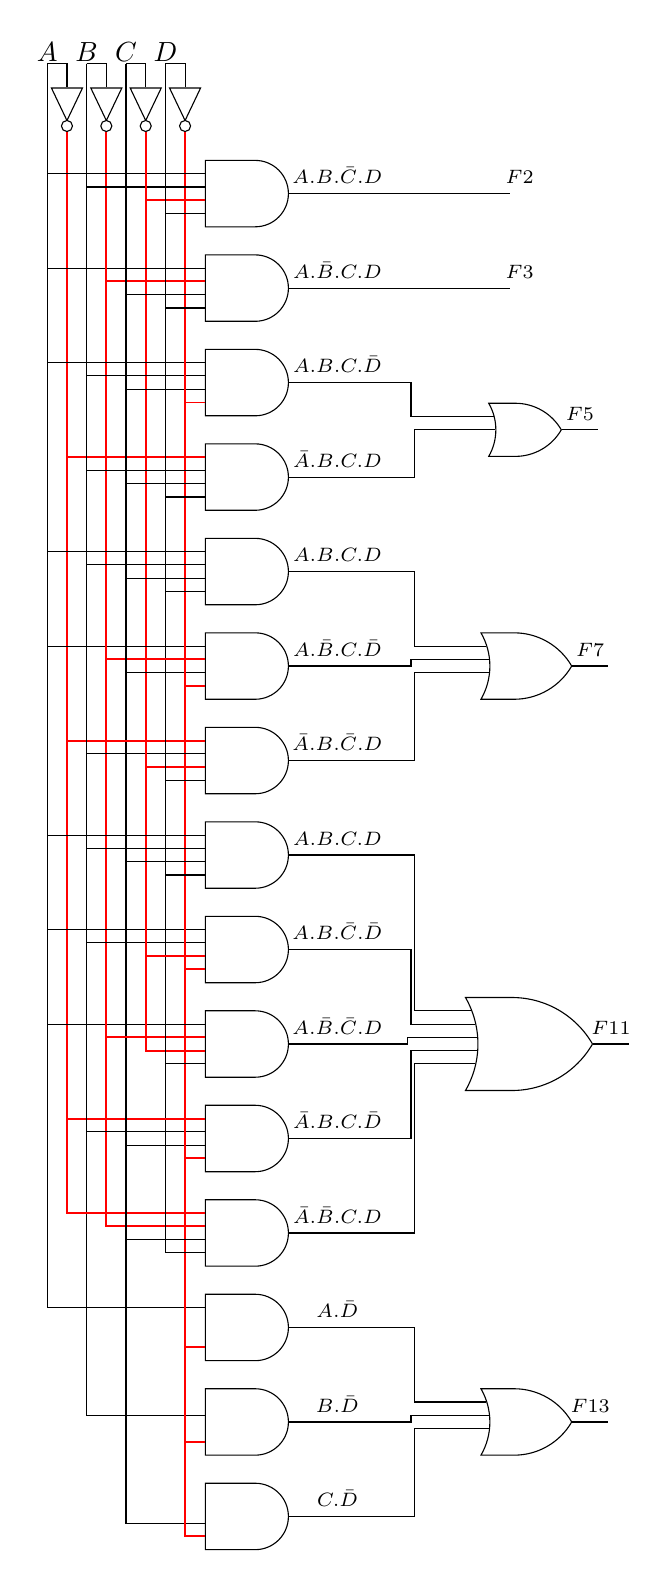
\begin{tikzpicture}

 %%Paramaters
%% var position, can be modified
\def\varPos{19.80}
\def\FunctionPos{6}
\node (x) at (0, \varPos) {$A$};
\node (y) at (0.5, \varPos) {$B$};
\node (z) at (1, \varPos) {$C$};
\node (w) at (1.5, \varPos) {$D$};

                \node[not gate US, draw, rotate=270] at ($(x) + (0.25, -0.6)$) (notx) {};
                \draw ($(x)+(0,-1ex)$) -| (notx.input); 
                \node[not gate US, draw, rotate=270] at ($(y) + (0.25, -0.6)$) (noty) {};
                \draw ($(y)+(0,-1ex)$) -| (noty.input); 
                \node[not gate US, draw, rotate=270] at ($(z) + (0.25, -0.6)$) (notz) {};
                \draw ($(z)+(0,-1ex)$) -| (notz.input);
                \node[not gate US, draw, rotate=270] at ($(w) + (0.25, -0.6)$) (notw) {};
                \draw ($(w)+(0,-1ex)$) -| (notw.input);
             

 %% ***Function F13 : Gate for term n° 1 [ C.D' ]***
  
                \node[and gate US, draw, rotate=0, logic gate inputs=nnnn] at (2.5, 1.20) (xandy1) {};\draw (xandy1.output) -- node[above]{\scriptsize $ C.\bar D $} ($(xandy1) + (1.8, 0)$);
                % Z
\draw ($(z) + (0, -1ex)$)|- (xandy1.input 3);
% W
\draw [line width=0.25mm,   red] (notw.output)
            -- ([xshift=0cm]notw.output) |- (xandy1.input 4);
 

 %% ***Function F13 : Gate for term n° 2 [ B.D' ]***
  
                \node[and gate US, draw, rotate=0, logic gate inputs=nnnn] at (2.5, 2.40) (xandy2) {};\draw (xandy2.output) -- node[above]{\scriptsize $ B.\bar D $} ($(xandy2) + (1.8, 0)$);
                % Y
\draw ($(y) + (0, -1ex)$)|- (xandy2.input 2);
% W
\draw [line width=0.25mm,   red] (notw.output)
            -- ([xshift=0cm]notw.output) |- (xandy2.input 4);
 

 %% ***Function F13 : Gate for term n° 3 [ A.D' ]***
  
                \node[and gate US, draw, rotate=0, logic gate inputs=nnnn] at (2.5, 3.60) (xandy3) {};\draw (xandy3.output) -- node[above]{\scriptsize $ A.\bar D $} ($(xandy3) + (1.8, 0)$);
                % X
\draw ($(x) + (0, -1ex)$)|- (xandy3.input 1);
% W
\draw [line width=0.25mm,   red] (notw.output)
            -- ([xshift=0cm]notw.output) |- (xandy3.input 4);


%% Function F13 Large OR Gate

\node[or gate US, draw, rotate=0, logic gate inputs=nnnn] at (\FunctionPos, 2.40) (xory1) {};


            \draw (xory1.output) -- node[above]{\scriptsize $F13$} ($(xory1.east) + (+3ex, 0)$);


            \draw (xandy1.output) -- ([xshift=1.60cm]xandy1.output) |- (xory1.input 3);

\draw (xandy2.output) -- ([xshift=1.55cm]xandy2.output) |- (xory1.input 2);

\draw (xandy3.output) -- ([xshift=1.60cm]xandy3.output) |- (xory1.input 1);

 

 %% ***Function F11 : Gate for term n° 1 [ A'.B'.C.D ]***
  
                \node[and gate US, draw, rotate=0, logic gate inputs=nnnn] at (2.5, 4.80) (xandy4) {};\draw (xandy4.output) -- node[above]{\scriptsize $ \bar A.\bar B.C.D $} ($(xandy4) + (1.8, 0)$);
                % X
\draw [line width=0.25mm,   red] (notx.output)
            -- ([xshift=0cm]notx.output) |- (xandy4.input 1);
% Y
\draw [line width=0.25mm,   red] (noty.output)
            -- ([xshift=0cm]noty.output) |- (xandy4.input 2);
% Z
\draw ($(z) + (0, -1ex)$)|- (xandy4.input 3);
% W
\draw ($(w) + (0, -1ex)$)|- (xandy4.input 4);
 

 %% ***Function F11 : Gate for term n° 2 [ A'.B.C.D' ]***
  
                \node[and gate US, draw, rotate=0, logic gate inputs=nnnn] at (2.5, 6.00) (xandy5) {};\draw (xandy5.output) -- node[above]{\scriptsize $ \bar A.B.C.\bar D $} ($(xandy5) + (1.8, 0)$);
                % X
\draw [line width=0.25mm,   red] (notx.output)
            -- ([xshift=0cm]notx.output) |- (xandy5.input 1);
% Y
\draw ($(y) + (0, -1ex)$)|- (xandy5.input 2);
% Z
\draw ($(z) + (0, -1ex)$)|- (xandy5.input 3);
% W
\draw [line width=0.25mm,   red] (notw.output)
            -- ([xshift=0cm]notw.output) |- (xandy5.input 4);
 

 %% ***Function F11 : Gate for term n° 3 [ A.B'.C'.D ]***
  
                \node[and gate US, draw, rotate=0, logic gate inputs=nnnn] at (2.5, 7.20) (xandy6) {};\draw (xandy6.output) -- node[above]{\scriptsize $ A.\bar B.\bar C.D $} ($(xandy6) + (1.8, 0)$);
                % X
\draw ($(x) + (0, -1ex)$)|- (xandy6.input 1);
% Y
\draw [line width=0.25mm,   red] (noty.output)
            -- ([xshift=0cm]noty.output) |- (xandy6.input 2);
% Z
\draw [line width=0.25mm,   red] (notz.output)
            -- ([xshift=0cm]notz.output) |- (xandy6.input 3);
% W
\draw ($(w) + (0, -1ex)$)|- (xandy6.input 4);
 

 %% ***Function F11 : Gate for term n° 4 [ A.B.C'.D' ]***
  
                \node[and gate US, draw, rotate=0, logic gate inputs=nnnn] at (2.5, 8.40) (xandy7) {};\draw (xandy7.output) -- node[above]{\scriptsize $ A.B.\bar C.\bar D $} ($(xandy7) + (1.8, 0)$);
                % X
\draw ($(x) + (0, -1ex)$)|- (xandy7.input 1);
% Y
\draw ($(y) + (0, -1ex)$)|- (xandy7.input 2);
% Z
\draw [line width=0.25mm,   red] (notz.output)
            -- ([xshift=0cm]notz.output) |- (xandy7.input 3);
% W
\draw [line width=0.25mm,   red] (notw.output)
            -- ([xshift=0cm]notw.output) |- (xandy7.input 4);
 

 %% ***Function F11 : Gate for term n° 5 [ A.B.C.D ]***
  
                \node[and gate US, draw, rotate=0, logic gate inputs=nnnn] at (2.5, 9.60) (xandy8) {};\draw (xandy8.output) -- node[above]{\scriptsize $ A.B.C.D $} ($(xandy8) + (1.8, 0)$);
                % X
\draw ($(x) + (0, -1ex)$)|- (xandy8.input 1);
% Y
\draw ($(y) + (0, -1ex)$)|- (xandy8.input 2);
% Z
\draw ($(z) + (0, -1ex)$)|- (xandy8.input 3);
% W
\draw ($(w) + (0, -1ex)$)|- (xandy8.input 4);


%% Function F11 Large OR Gate

\node[or gate US, draw, rotate=0, logic gate inputs=nnnnnn] at (\FunctionPos, 7.20) (xory4) {};


            \draw (xory4.output) -- node[above]{\scriptsize $F11$} ($(xory4.east) + (+3ex, 0)$);


            \draw (xandy4.output) -- ([xshift=1.60cm]xandy4.output) |- (xory4.input 5);

\draw (xandy5.output) -- ([xshift=1.55cm]xandy5.output) |- (xory4.input 4);

\draw (xandy6.output) -- ([xshift=1.50cm]xandy6.output) |- (xory4.input 3);

\draw (xandy7.output) -- ([xshift=1.55cm]xandy7.output) |- (xory4.input 2);

\draw (xandy8.output) -- ([xshift=1.60cm]xandy8.output) |- (xory4.input 1);

 

 %% ***Function F7 : Gate for term n° 1 [ A'.B.C'.D ]***
  
                \node[and gate US, draw, rotate=0, logic gate inputs=nnnn] at (2.5, 10.80) (xandy9) {};\draw (xandy9.output) -- node[above]{\scriptsize $ \bar A.B.\bar C.D $} ($(xandy9) + (1.8, 0)$);
                % X
\draw [line width=0.25mm,   red] (notx.output)
            -- ([xshift=0cm]notx.output) |- (xandy9.input 1);
% Y
\draw ($(y) + (0, -1ex)$)|- (xandy9.input 2);
% Z
\draw [line width=0.25mm,   red] (notz.output)
            -- ([xshift=0cm]notz.output) |- (xandy9.input 3);
% W
\draw ($(w) + (0, -1ex)$)|- (xandy9.input 4);
 

 %% ***Function F7 : Gate for term n° 2 [ A.B'.C.D' ]***
  
                \node[and gate US, draw, rotate=0, logic gate inputs=nnnn] at (2.5, 12.00) (xandy10) {};\draw (xandy10.output) -- node[above]{\scriptsize $ A.\bar B.C.\bar D $} ($(xandy10) + (1.8, 0)$);
                % X
\draw ($(x) + (0, -1ex)$)|- (xandy10.input 1);
% Y
\draw [line width=0.25mm,   red] (noty.output)
            -- ([xshift=0cm]noty.output) |- (xandy10.input 2);
% Z
\draw ($(z) + (0, -1ex)$)|- (xandy10.input 3);
% W
\draw [line width=0.25mm,   red] (notw.output)
            -- ([xshift=0cm]notw.output) |- (xandy10.input 4);
 

 %% ***Function F7 : Gate for term n° 3 [ A.B.C.D ]***
  
                \node[and gate US, draw, rotate=0, logic gate inputs=nnnn] at (2.5, 13.20) (xandy11) {};\draw (xandy11.output) -- node[above]{\scriptsize $ A.B.C.D $} ($(xandy11) + (1.8, 0)$);
                % X
\draw ($(x) + (0, -1ex)$)|- (xandy11.input 1);
% Y
\draw ($(y) + (0, -1ex)$)|- (xandy11.input 2);
% Z
\draw ($(z) + (0, -1ex)$)|- (xandy11.input 3);
% W
\draw ($(w) + (0, -1ex)$)|- (xandy11.input 4);


%% Function F7 Large OR Gate

\node[or gate US, draw, rotate=0, logic gate inputs=nnnn] at (\FunctionPos, 12.00) (xory9) {};


            \draw (xory9.output) -- node[above]{\scriptsize $F7$} ($(xory9.east) + (+3ex, 0)$);


            \draw (xandy9.output) -- ([xshift=1.60cm]xandy9.output) |- (xory9.input 3);

\draw (xandy10.output) -- ([xshift=1.55cm]xandy10.output) |- (xory9.input 2);

\draw (xandy11.output) -- ([xshift=1.60cm]xandy11.output) |- (xory9.input 1);

 

 %% ***Function F5 : Gate for term n° 1 [ A'.B.C.D ]***
  
                \node[and gate US, draw, rotate=0, logic gate inputs=nnnn] at (2.5, 14.40) (xandy12) {};\draw (xandy12.output) -- node[above]{\scriptsize $ \bar A.B.C.D $} ($(xandy12) + (1.8, 0)$);
                % X
\draw [line width=0.25mm,   red] (notx.output)
            -- ([xshift=0cm]notx.output) |- (xandy12.input 1);
% Y
\draw ($(y) + (0, -1ex)$)|- (xandy12.input 2);
% Z
\draw ($(z) + (0, -1ex)$)|- (xandy12.input 3);
% W
\draw ($(w) + (0, -1ex)$)|- (xandy12.input 4);
 

 %% ***Function F5 : Gate for term n° 2 [ A.B.C.D' ]***
  
                \node[and gate US, draw, rotate=0, logic gate inputs=nnnn] at (2.5, 15.60) (xandy13) {};\draw (xandy13.output) -- node[above]{\scriptsize $ A.B.C.\bar D $} ($(xandy13) + (1.8, 0)$);
                % X
\draw ($(x) + (0, -1ex)$)|- (xandy13.input 1);
% Y
\draw ($(y) + (0, -1ex)$)|- (xandy13.input 2);
% Z
\draw ($(z) + (0, -1ex)$)|- (xandy13.input 3);
% W
\draw [line width=0.25mm,   red] (notw.output)
            -- ([xshift=0cm]notw.output) |- (xandy13.input 4);


%% Function F5 Large OR Gate

\node[or gate US, draw, rotate=0, logic gate inputs=nnn] at (\FunctionPos, 15.00) (xory12) {};


            \draw (xory12.output) -- node[above]{\scriptsize $F5$} ($(xory12.east) + (+3ex, 0)$);


            \draw (xandy12.output) -- ([xshift=1.60cm]xandy12.output) |- (xory12.input 2);

\draw (xandy13.output) -- ([xshift=1.55cm]xandy13.output) |- (xory12.input 1);

 

 %% ***Function F3 : Gate for term n° 1 [ A.B'.C.D ]***
  
                \node[and gate US, draw, rotate=0, logic gate inputs=nnnn] at (2.5, 16.80) (xandy14) {};\draw (xandy14.output) -- node[above]{\scriptsize $ A.\bar B.C.D $} ($(xandy14) + (1.8, 0)$);
                % X
\draw ($(x) + (0, -1ex)$)|- (xandy14.input 1);
% Y
\draw [line width=0.25mm,   red] (noty.output)
            -- ([xshift=0cm]noty.output) |- (xandy14.input 2);
% Z
\draw ($(z) + (0, -1ex)$)|- (xandy14.input 3);
% W
\draw ($(w) + (0, -1ex)$)|- (xandy14.input 4);


%% Function F3 Large OR Gate

\node at (\FunctionPos, 16.80) (xory14) {};


            \draw (xory14) node[above]{\scriptsize $F3$} ($(xory14.east) + (+3ex, 0)$);


            \draw (xandy14.output) -- ([xshift=1.60cm]xandy14.output) |- (xory14);

 

 %% ***Function F2 : Gate for term n° 1 [ A.B.C'.D ]***
  
                \node[and gate US, draw, rotate=0, logic gate inputs=nnnn] at (2.5, 18.00) (xandy15) {};\draw (xandy15.output) -- node[above]{\scriptsize $ A.B.\bar C.D $} ($(xandy15) + (1.8, 0)$);
                % X
\draw ($(x) + (0, -1ex)$)|- (xandy15.input 1);
% Y
\draw ($(y) + (0, -1ex)$)|- (xandy15.input 2);
% Z
\draw [line width=0.25mm,   red] (notz.output)
            -- ([xshift=0cm]notz.output) |- (xandy15.input 3);
% W
\draw ($(w) + (0, -1ex)$)|- (xandy15.input 4);


%% Function F2 Large OR Gate

\node at (\FunctionPos, 18.00) (xory15) {};


            \draw (xory15) node[above]{\scriptsize $F2$} ($(xory15.east) + (+3ex, 0)$);


            \draw (xandy15.output) -- ([xshift=1.60cm]xandy15.output) |- (xory15);

 \end{tikzpicture}



LOGIGRAM-FILE-TEMPLATE




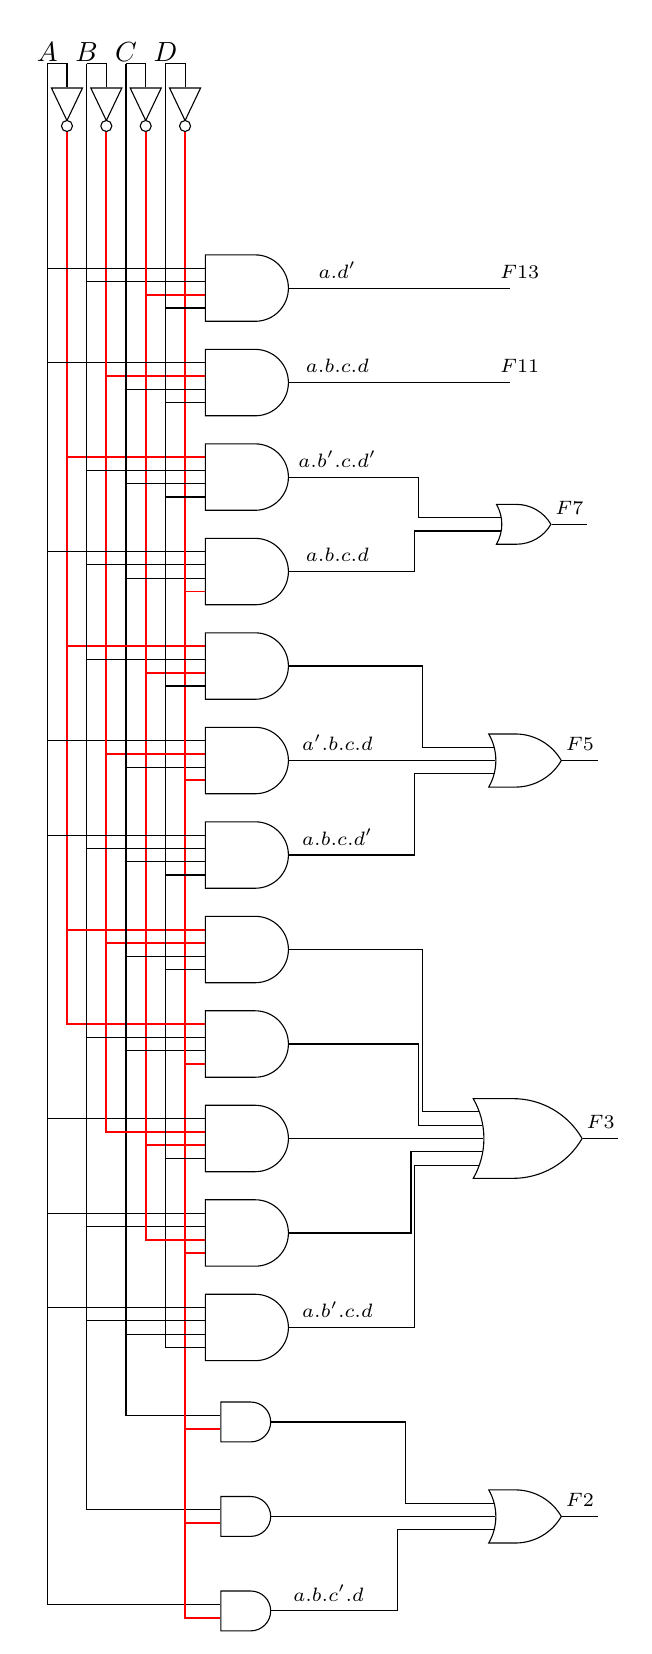
\begin{tikzpicture}

%%Paramaters
%% var position, can be modified


  

  

  

  

  

  

\def\varPos{ 19.8 }



\def\FunctionPos{6}



    \node (x1) at (0.0, \varPos) {$ A $};
    \node[not gate US, draw, rotate=270] at ($(x1) + (0.25, -0.6)$) (notx1) {};
    \draw ($(x1)+(0,-1ex)$) -| (notx1.input);

    \node (x2) at (0.5, \varPos) {$ B $};
    \node[not gate US, draw, rotate=270] at ($(x2) + (0.25, -0.6)$) (notx2) {};
    \draw ($(x2)+(0,-1ex)$) -| (notx2.input);

    \node (x3) at (1.0, \varPos) {$ C $};
    \node[not gate US, draw, rotate=270] at ($(x3) + (0.25, -0.6)$) (notx3) {};
    \draw ($(x3)+(0,-1ex)$) -| (notx3.input);

    \node (x4) at (1.5, \varPos) {$ D $};
    \node[not gate US, draw, rotate=270] at ($(x4) + (0.25, -0.6)$) (notx4) {};
    \draw ($(x4)+(0,-1ex)$) -| (notx4.input);







    
    
    

    
        
        
        
        
        
     %% ***Function F2 : Gate for term n° 1 [  a.b.c'.d  ]***

           \node[and gate US, draw, rotate=0, logic gate inputs=nn] at (2.5, 0.0) (xandyF21) {};
           \draw (xandyF21.output) -- node[above]{\scriptsize $  a.b.c'.d  $} ($(xandyF21) + (1.8, 0)$);

        
        
            
                \draw ($(x1) + (0, -1ex)$)|- (xandyF21.input 1);
                
            
        
            
        
            
        
            
                \draw [line width=0.25mm,   red] (notx4.output)
                -- ([xshift=0cm]notx4.output) |- (xandyF21.input 2);
                
            
        
     
    
        
        
        
        
        
     %% ***Function F2 : Gate for term n° 2 [  ]***

           \node[and gate US, draw, rotate=0, logic gate inputs=nn] at (2.5, 1.2) (xandyF22) {};
           \draw (xandyF22.output) -- node[above]{\scriptsize $  $} ($(xandyF22) + (1.8, 0)$);

        
        
            
        
            
                \draw ($(x2) + (0, -1ex)$)|- (xandyF22.input 1);
                
            
        
            
        
            
                \draw [line width=0.25mm,   red] (notx4.output)
                -- ([xshift=0cm]notx4.output) |- (xandyF22.input 2);
                
            
        
     
    
        
        
        
        
        
     %% ***Function F2 : Gate for term n° 3 [  ]***

           \node[and gate US, draw, rotate=0, logic gate inputs=nn] at (2.5, 2.4) (xandyF23) {};
           \draw (xandyF23.output) -- node[above]{\scriptsize $  $} ($(xandyF23) + (1.8, 0)$);

        
        
            
        
            
        
            
                \draw ($(x3) + (0, -1ex)$)|- (xandyF23.input 1);
                
            
        
            
                \draw [line width=0.25mm,   red] (notx4.output)
                -- ([xshift=0cm]notx4.output) |- (xandyF23.input 2);
                
            
        
     
    


    %% y_pos : the position of OR gate according to their related gates
    

    %% Function F2 Large OR Gate
    
        \node[or gate US, draw, rotate=0, logic gate inputs=nnn] at (\FunctionPos, 1.2) (xoryF2) {};
        \draw (xoryF2.output) -- node[above]{\scriptsize $F2$} ($(xoryF2.east) + (+3ex, 0)$);
    


    
    
    
    
        
             \draw (xandyF21.output) -- ([xshift=1.6cm]xandyF21.output) |- (xoryF2.input 3);
        
        
            
        
    
        
             \draw (xandyF22.output) -- ([xshift=1.6500000000000001cm]xandyF22.output) |- (xoryF2.input 2);
        
        
            
        
    
        
             \draw (xandyF23.output) -- ([xshift=1.7000000000000002cm]xandyF23.output) |- (xoryF2.input 1);
        
        
            
        
    

    
    
    

    
        
        
        
        
        
     %% ***Function F3 : Gate for term n° 1 [  a.b'.c.d  ]***

           \node[and gate US, draw, rotate=0, logic gate inputs=nnnn] at (2.5, 3.5999999999999996) (xandyF31) {};
           \draw (xandyF31.output) -- node[above]{\scriptsize $  a.b'.c.d  $} ($(xandyF31) + (1.8, 0)$);

        
        
            
                \draw ($(x1) + (0, -1ex)$)|- (xandyF31.input 1);
                
            
        
            
                \draw ($(x2) + (0, -1ex)$)|- (xandyF31.input 2);
                
            
        
            
                \draw ($(x3) + (0, -1ex)$)|- (xandyF31.input 3);
                
            
        
            
                \draw ($(x4) + (0, -1ex)$)|- (xandyF31.input 4);
                
            
        
     
    
        
        
        
        
        
     %% ***Function F3 : Gate for term n° 2 [  ]***

           \node[and gate US, draw, rotate=0, logic gate inputs=nnnn] at (2.5, 4.8) (xandyF32) {};
           \draw (xandyF32.output) -- node[above]{\scriptsize $  $} ($(xandyF32) + (1.8, 0)$);

        
        
            
                \draw ($(x1) + (0, -1ex)$)|- (xandyF32.input 1);
                
            
        
            
                \draw ($(x2) + (0, -1ex)$)|- (xandyF32.input 2);
                
            
        
            
                \draw [line width=0.25mm,   red] (notx3.output)
                -- ([xshift=0cm]notx3.output) |- (xandyF32.input 3);
                
            
        
            
                \draw [line width=0.25mm,   red] (notx4.output)
                -- ([xshift=0cm]notx4.output) |- (xandyF32.input 4);
                
            
        
     
    
        
        
        
        
        
     %% ***Function F3 : Gate for term n° 3 [  ]***

           \node[and gate US, draw, rotate=0, logic gate inputs=nnnn] at (2.5, 6.0) (xandyF33) {};
           \draw (xandyF33.output) -- node[above]{\scriptsize $  $} ($(xandyF33) + (1.8, 0)$);

        
        
            
                \draw ($(x1) + (0, -1ex)$)|- (xandyF33.input 1);
                
            
        
            
                \draw [line width=0.25mm,   red] (notx2.output)
                -- ([xshift=0cm]notx2.output) |- (xandyF33.input 2);
                
            
        
            
                \draw [line width=0.25mm,   red] (notx3.output)
                -- ([xshift=0cm]notx3.output) |- (xandyF33.input 3);
                
            
        
            
                \draw ($(x4) + (0, -1ex)$)|- (xandyF33.input 4);
                
            
        
     
    
        
        
        
        
        
     %% ***Function F3 : Gate for term n° 4 [  ]***

           \node[and gate US, draw, rotate=0, logic gate inputs=nnnn] at (2.5, 7.199999999999999) (xandyF34) {};
           \draw (xandyF34.output) -- node[above]{\scriptsize $  $} ($(xandyF34) + (1.8, 0)$);

        
        
            
                \draw [line width=0.25mm,   red] (notx1.output)
                -- ([xshift=0cm]notx1.output) |- (xandyF34.input 1);
                
            
        
            
                \draw ($(x2) + (0, -1ex)$)|- (xandyF34.input 2);
                
            
        
            
                \draw ($(x3) + (0, -1ex)$)|- (xandyF34.input 3);
                
            
        
            
                \draw [line width=0.25mm,   red] (notx4.output)
                -- ([xshift=0cm]notx4.output) |- (xandyF34.input 4);
                
            
        
     
    
        
        
        
        
        
     %% ***Function F3 : Gate for term n° 5 [  ]***

           \node[and gate US, draw, rotate=0, logic gate inputs=nnnn] at (2.5, 8.4) (xandyF35) {};
           \draw (xandyF35.output) -- node[above]{\scriptsize $  $} ($(xandyF35) + (1.8, 0)$);

        
        
            
                \draw [line width=0.25mm,   red] (notx1.output)
                -- ([xshift=0cm]notx1.output) |- (xandyF35.input 1);
                
            
        
            
                \draw [line width=0.25mm,   red] (notx2.output)
                -- ([xshift=0cm]notx2.output) |- (xandyF35.input 2);
                
            
        
            
                \draw ($(x3) + (0, -1ex)$)|- (xandyF35.input 3);
                
            
        
            
                \draw ($(x4) + (0, -1ex)$)|- (xandyF35.input 4);
                
            
        
     
    


    %% y_pos : the position of OR gate according to their related gates
    

    %% Function F3 Large OR Gate
    
        \node[or gate US, draw, rotate=0, logic gate inputs=nnnnn] at (\FunctionPos, 6.0) (xoryF3) {};
        \draw (xoryF3.output) -- node[above]{\scriptsize $F3$} ($(xoryF3.east) + (+3ex, 0)$);
    


    
    
    
    
        
             \draw (xandyF31.output) -- ([xshift=1.6cm]xandyF31.output) |- (xoryF3.input 5);
        
        
            
        
    
        
             \draw (xandyF32.output) -- ([xshift=1.55cm]xandyF32.output) |- (xoryF3.input 4);
        
        
            
        
    
        
             \draw (xandyF33.output) -- ([xshift=1.6cm]xandyF33.output) |- (xoryF3.input 3);
        
        
            
        
    
        
             \draw (xandyF34.output) -- ([xshift=1.6500000000000001cm]xandyF34.output) |- (xoryF3.input 2);
        
        
            
        
    
        
             \draw (xandyF35.output) -- ([xshift=1.7000000000000002cm]xandyF35.output) |- (xoryF3.input 1);
        
        
            
        
    

    
    
    

    
        
        
        
        
        
     %% ***Function F5 : Gate for term n° 1 [  a.b.c.d'  ]***

           \node[and gate US, draw, rotate=0, logic gate inputs=nnnn] at (2.5, 9.6) (xandyF51) {};
           \draw (xandyF51.output) -- node[above]{\scriptsize $  a.b.c.d'  $} ($(xandyF51) + (1.8, 0)$);

        
        
            
                \draw ($(x1) + (0, -1ex)$)|- (xandyF51.input 1);
                
            
        
            
                \draw ($(x2) + (0, -1ex)$)|- (xandyF51.input 2);
                
            
        
            
                \draw ($(x3) + (0, -1ex)$)|- (xandyF51.input 3);
                
            
        
            
                \draw ($(x4) + (0, -1ex)$)|- (xandyF51.input 4);
                
            
        
     
    
        
        
        
        
        
     %% ***Function F5 : Gate for term n° 2 [  a'.b.c.d  ]***

           \node[and gate US, draw, rotate=0, logic gate inputs=nnnn] at (2.5, 10.799999999999999) (xandyF52) {};
           \draw (xandyF52.output) -- node[above]{\scriptsize $  a'.b.c.d  $} ($(xandyF52) + (1.8, 0)$);

        
        
            
                \draw ($(x1) + (0, -1ex)$)|- (xandyF52.input 1);
                
            
        
            
                \draw [line width=0.25mm,   red] (notx2.output)
                -- ([xshift=0cm]notx2.output) |- (xandyF52.input 2);
                
            
        
            
                \draw ($(x3) + (0, -1ex)$)|- (xandyF52.input 3);
                
            
        
            
                \draw [line width=0.25mm,   red] (notx4.output)
                -- ([xshift=0cm]notx4.output) |- (xandyF52.input 4);
                
            
        
     
    
        
        
        
        
        
     %% ***Function F5 : Gate for term n° 3 [  ]***

           \node[and gate US, draw, rotate=0, logic gate inputs=nnnn] at (2.5, 12.0) (xandyF53) {};
           \draw (xandyF53.output) -- node[above]{\scriptsize $  $} ($(xandyF53) + (1.8, 0)$);

        
        
            
                \draw [line width=0.25mm,   red] (notx1.output)
                -- ([xshift=0cm]notx1.output) |- (xandyF53.input 1);
                
            
        
            
                \draw ($(x2) + (0, -1ex)$)|- (xandyF53.input 2);
                
            
        
            
                \draw [line width=0.25mm,   red] (notx3.output)
                -- ([xshift=0cm]notx3.output) |- (xandyF53.input 3);
                
            
        
            
                \draw ($(x4) + (0, -1ex)$)|- (xandyF53.input 4);
                
            
        
     
    


    %% y_pos : the position of OR gate according to their related gates
    

    %% Function F5 Large OR Gate
    
        \node[or gate US, draw, rotate=0, logic gate inputs=nnn] at (\FunctionPos, 10.799999999999999) (xoryF5) {};
        \draw (xoryF5.output) -- node[above]{\scriptsize $F5$} ($(xoryF5.east) + (+3ex, 0)$);
    


    
    
    
    
        
             \draw (xandyF51.output) -- ([xshift=1.6cm]xandyF51.output) |- (xoryF5.input 3);
        
        
            
        
    
        
             \draw (xandyF52.output) -- ([xshift=1.6500000000000001cm]xandyF52.output) |- (xoryF5.input 2);
        
        
            
        
    
        
             \draw (xandyF53.output) -- ([xshift=1.7000000000000002cm]xandyF53.output) |- (xoryF5.input 1);
        
        
            
        
    

    
    
    

    
        
        
        
        
        
     %% ***Function F7 : Gate for term n° 1 [  a.b.c.d  ]***

           \node[and gate US, draw, rotate=0, logic gate inputs=nnnn] at (2.5, 13.2) (xandyF71) {};
           \draw (xandyF71.output) -- node[above]{\scriptsize $  a.b.c.d  $} ($(xandyF71) + (1.8, 0)$);

        
        
            
                \draw ($(x1) + (0, -1ex)$)|- (xandyF71.input 1);
                
            
        
            
                \draw ($(x2) + (0, -1ex)$)|- (xandyF71.input 2);
                
            
        
            
                \draw ($(x3) + (0, -1ex)$)|- (xandyF71.input 3);
                
            
        
            
                \draw [line width=0.25mm,   red] (notx4.output)
                -- ([xshift=0cm]notx4.output) |- (xandyF71.input 4);
                
            
        
     
    
        
        
        
        
        
     %% ***Function F7 : Gate for term n° 2 [  a.b'.c.d'  ]***

           \node[and gate US, draw, rotate=0, logic gate inputs=nnnn] at (2.5, 14.399999999999999) (xandyF72) {};
           \draw (xandyF72.output) -- node[above]{\scriptsize $  a.b'.c.d'  $} ($(xandyF72) + (1.8, 0)$);

        
        
            
                \draw [line width=0.25mm,   red] (notx1.output)
                -- ([xshift=0cm]notx1.output) |- (xandyF72.input 1);
                
            
        
            
                \draw ($(x2) + (0, -1ex)$)|- (xandyF72.input 2);
                
            
        
            
                \draw ($(x3) + (0, -1ex)$)|- (xandyF72.input 3);
                
            
        
            
                \draw ($(x4) + (0, -1ex)$)|- (xandyF72.input 4);
                
            
        
     
    


    %% y_pos : the position of OR gate according to their related gates
    

    %% Function F7 Large OR Gate
    
        \node[or gate US, draw, rotate=0, logic gate inputs=nn] at (\FunctionPos, 13.799999999999999) (xoryF7) {};
        \draw (xoryF7.output) -- node[above]{\scriptsize $F7$} ($(xoryF7.east) + (+3ex, 0)$);
    


    
    
    
    
        
             \draw (xandyF71.output) -- ([xshift=1.6cm]xandyF71.output) |- (xoryF7.input 2);
        
        
            
        
    
        
             \draw (xandyF72.output) -- ([xshift=1.6500000000000001cm]xandyF72.output) |- (xoryF7.input 1);
        
        
            
        
    

    
    
    

    
        
        
        
        
        
     %% ***Function F11 : Gate for term n° 1 [  a.b.c.d  ]***

           \node[and gate US, draw, rotate=0, logic gate inputs=nnnn] at (2.5, 15.6) (xandyF111) {};
           \draw (xandyF111.output) -- node[above]{\scriptsize $  a.b.c.d  $} ($(xandyF111) + (1.8, 0)$);

        
        
            
                \draw ($(x1) + (0, -1ex)$)|- (xandyF111.input 1);
                
            
        
            
                \draw [line width=0.25mm,   red] (notx2.output)
                -- ([xshift=0cm]notx2.output) |- (xandyF111.input 2);
                
            
        
            
                \draw ($(x3) + (0, -1ex)$)|- (xandyF111.input 3);
                
            
        
            
                \draw ($(x4) + (0, -1ex)$)|- (xandyF111.input 4);
                
            
        
     
    


    %% y_pos : the position of OR gate according to their related gates
    

    %% Function F11 Large OR Gate
    
        \node at (\FunctionPos, 15.6) (xoryF11) {};
        \draw (xoryF11)  node[above]{\scriptsize $F11$} ($(xoryF11.east) + (+3ex, 0)$);
    


    
    
    
    
        
             \draw (xandyF111.output) -- ([xshift=1.6cm]xandyF111.output) |- (xoryF11);
        
        
            
        
    

    
    
    

    
        
        
        
        
        
     %% ***Function F13 : Gate for term n° 1 [  a.d'  ]***

           \node[and gate US, draw, rotate=0, logic gate inputs=nnnn] at (2.5, 16.8) (xandyF131) {};
           \draw (xandyF131.output) -- node[above]{\scriptsize $  a.d'  $} ($(xandyF131) + (1.8, 0)$);

        
        
            
                \draw ($(x1) + (0, -1ex)$)|- (xandyF131.input 1);
                
            
        
            
                \draw ($(x2) + (0, -1ex)$)|- (xandyF131.input 2);
                
            
        
            
                \draw [line width=0.25mm,   red] (notx3.output)
                -- ([xshift=0cm]notx3.output) |- (xandyF131.input 3);
                
            
        
            
                \draw ($(x4) + (0, -1ex)$)|- (xandyF131.input 4);
                
            
        
     
    


    %% y_pos : the position of OR gate according to their related gates
    

    %% Function F13 Large OR Gate
    
        \node at (\FunctionPos, 16.8) (xoryF13) {};
        \draw (xoryF13)  node[above]{\scriptsize $F13$} ($(xoryF13.east) + (+3ex, 0)$);
    


    
    
    
    
        
             \draw (xandyF131.output) -- ([xshift=1.6cm]xandyF131.output) |- (xoryF13);
        
        
            
        
    


 \end{tikzpicture}

STRUCTURED LOGIGRAM-FILE-TEMPLATE
\begin{verbatim}
{'function_gate': 'or',
 'functions': [{'name': 'F13',
                'nb_terms': 1,
                'terms': [{'id': 'xandyF13g0',
                           'label': "A.B.C'.D",
                           'name': "A.B.C'.D",
                           'vars': ['A', 'B', "C'", 'D']}]},
               {'name': 'F11',
                'nb_terms': 1,
                'terms': [{'id': 'xandyF11g0',
                           'label': "A.B'.C.D",
                           'name': "A.B'.C.D",
                           'vars': ['A', "B'", 'C', 'D']}]},
               {'name': 'F7',
                'nb_terms': 2,
                'terms': [{'id': 'xandyF7g0',
                           'label': "A'.B.C.D",
                           'name': "A'.B.C.D",
                           'vars': ["A'", 'B', 'C', 'D']},
                          {'id': 'xandyF7g1',
                           'label': "A.B.C.D'",
                           'name': "A.B.C.D'",
                           'vars': ['A', 'B', 'C', "D'"]}]},
               {'name': 'F5',
                'nb_terms': 3,
                'terms': [{'id': 'xandyF5g0',
                           'label': "A'.B.C'.D",
                           'name': "A'.B.C'.D",
                           'vars': ["A'", 'B', "C'", 'D']},
                          {'id': 'xandyF5g1',
                           'label': "A.B'.C.D'",
                           'name': "A.B'.C.D'",
                           'vars': ['A', "B'", 'C', "D'"]},
                          {'id': 'xandyF5g2',
                           'label': 'A.B.C.D',
                           'name': 'A.B.C.D',
                           'vars': ['A', 'B', 'C', 'D']}]},
               {'name': 'F3',
                'nb_terms': 5,
                'terms': [{'id': 'xandyF3g0',
                           'label': "A'.B'.C.D",
                           'name': "A'.B'.C.D",
                           'vars': ["A'", "B'", 'C', 'D']},
                          {'id': 'xandyF3g1',
                           'label': "A'.B.C.D'",
                           'name': "A'.B.C.D'",
                           'vars': ["A'", 'B', 'C', "D'"]},
                          {'id': 'xandyF3g2',
                           'label': "A.B'.C'.D",
                           'name': "A.B'.C'.D",
                           'vars': ['A', "B'", "C'", 'D']},
                          {'id': 'xandyF3g3',
                           'label': "A.B.C'.D'",
                           'name': "A.B.C'.D'",
                           'vars': ['A', 'B', "C'", "D'"]},
                          {'id': 'xandyF3g4',
                           'label': 'A.B.C.D',
                           'name': 'A.B.C.D',
                           'vars': ['A', 'B', 'C', 'D']}]},
               {'name': 'F2',
                'nb_terms': 3,
                'terms': [{'id': 'xandyF2g0',
                           'label': "C.D'",
                           'name': "C.D'",
                           'vars': ['C', "D'"]},
                          {'id': 'xandyF2g1',
                           'label': "B.D'",
                           'name': "B.D'",
                           'vars': ['B', "D'"]},
                          {'id': 'xandyF2g2',
                           'label': "A.D'",
                           'name': "A.D'",
                           'vars': ['A', "D'"]}]}],
 'method': '',
 'size_terms': 15,
 'term_gate': 'and',
 'variables': ['A', 'B', 'C', 'D']}
\end{verbatim}





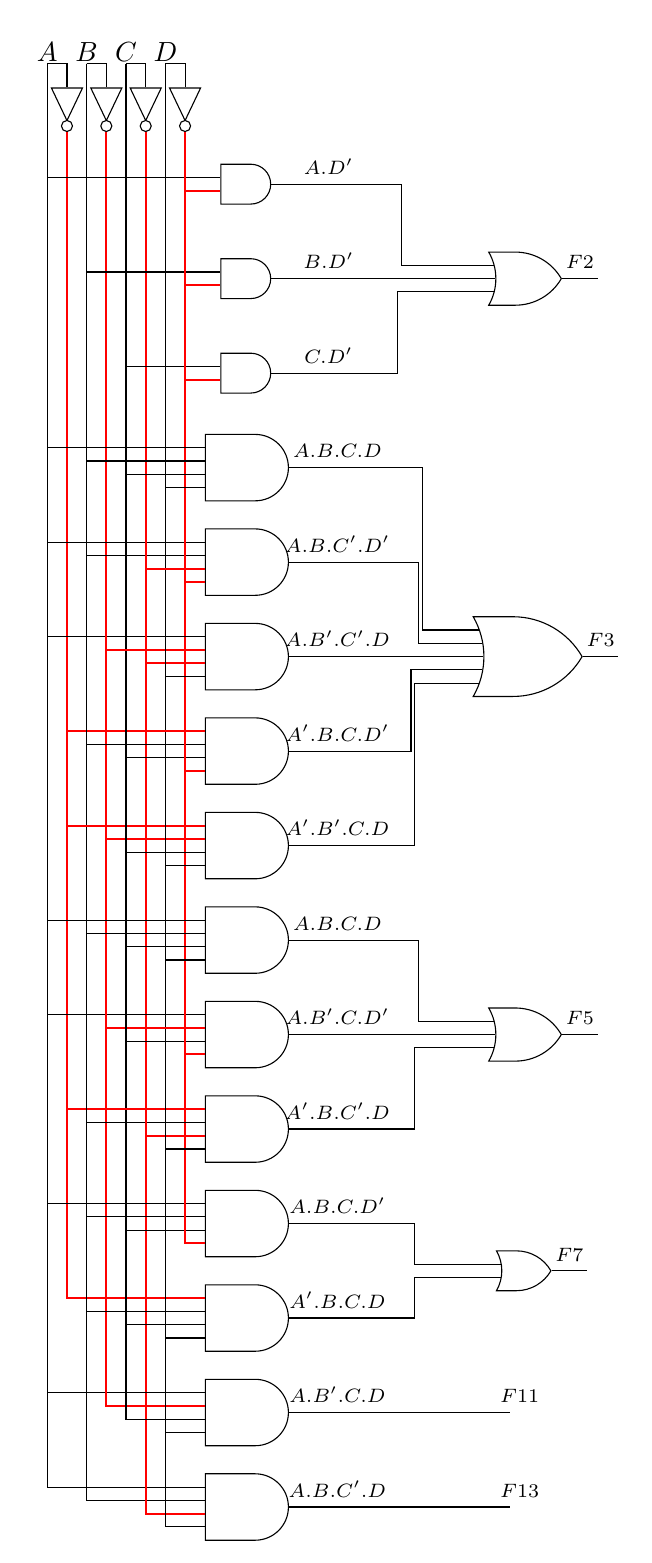
\begin{tikzpicture}

%%Paramaters
%% var position, can be modified
\def\varPos{ 18.48 }


\def\FunctionPos{6}



    \node (x1) at (0.0, \varPos) {$ A $};
    \node[not gate US, draw, rotate=270] at ($(x1) + (0.25, -0.6)$) (notx1) {};
    \draw ($(x1)+(0,-1ex)$) -| (notx1.input);

    \node (x2) at (0.5, \varPos) {$ B $};
    \node[not gate US, draw, rotate=270] at ($(x2) + (0.25, -0.6)$) (notx2) {};
    \draw ($(x2)+(0,-1ex)$) -| (notx2.input);

    \node (x3) at (1.0, \varPos) {$ C $};
    \node[not gate US, draw, rotate=270] at ($(x3) + (0.25, -0.6)$) (notx3) {};
    \draw ($(x3)+(0,-1ex)$) -| (notx3.input);

    \node (x4) at (1.5, \varPos) {$ D $};
    \node[not gate US, draw, rotate=270] at ($(x4) + (0.25, -0.6)$) (notx4) {};
    \draw ($(x4)+(0,-1ex)$) -| (notx4.input);








    
        
     %% ***Function F13 : Gate for term n° 1 [ A.B.C'.D ]***

           \node[and gate US, draw, rotate=0, logic gate inputs=nnnn] at (2.5, 0.0) (xandyF13g0) {};
           \draw (xandyF13g0.output) -- node[above]{\scriptsize $ A.B.C'.D $} ($(xandyF13g0) + (1.8, 0)$);

        
        
            
                \draw ($(x1) + (0, -1ex)$)|- (xandyF13g0.input 1);
                
            
        
            
                \draw ($(x2) + (0, -1ex)$)|- (xandyF13g0.input 2);
                
            
        
            
                \draw [line width=0.25mm,   red] (notx3.output)
                -- ([xshift=0cm]notx3.output) |- (xandyF13g0.input 3);
                
            
        
            
                \draw ($(x4) + (0, -1ex)$)|- (xandyF13g0.input 4);
                
            
        
     
    


    %% y_pos : the position of OR gate according to their related gates
    

    %% Function F13 Large OR Gate
    

    
        \node at (\FunctionPos, 0.0) (xoryF13) {};
        \draw (xoryF13)  node[above]{\scriptsize $F13$} ($(xoryF13.east) + (+3ex, 0)$);
    


    
    
    
    

        
             \draw (xandyF13g0.output) -- (xoryF13);
        
        

    

    
        
     %% ***Function F11 : Gate for term n° 1 [ A.B'.C.D ]***

           \node[and gate US, draw, rotate=0, logic gate inputs=nnnn] at (2.5, 1.2) (xandyF11g0) {};
           \draw (xandyF11g0.output) -- node[above]{\scriptsize $ A.B'.C.D $} ($(xandyF11g0) + (1.8, 0)$);

        
        
            
                \draw ($(x1) + (0, -1ex)$)|- (xandyF11g0.input 1);
                
            
        
            
                \draw [line width=0.25mm,   red] (notx2.output)
                -- ([xshift=0cm]notx2.output) |- (xandyF11g0.input 2);
                
            
        
            
                \draw ($(x3) + (0, -1ex)$)|- (xandyF11g0.input 3);
                
            
        
            
                \draw ($(x4) + (0, -1ex)$)|- (xandyF11g0.input 4);
                
            
        
     
    


    %% y_pos : the position of OR gate according to their related gates
    

    %% Function F11 Large OR Gate
    

    
        \node at (\FunctionPos, 1.2) (xoryF11) {};
        \draw (xoryF11)  node[above]{\scriptsize $F11$} ($(xoryF11.east) + (+3ex, 0)$);
    


    
    
    
    

        
             \draw (xandyF11g0.output) -- (xoryF11);
        
        

    

    
        
     %% ***Function F7 : Gate for term n° 1 [ A'.B.C.D ]***

           \node[and gate US, draw, rotate=0, logic gate inputs=nnnn] at (2.5, 2.4) (xandyF7g0) {};
           \draw (xandyF7g0.output) -- node[above]{\scriptsize $ A'.B.C.D $} ($(xandyF7g0) + (1.8, 0)$);

        
        
            
                \draw [line width=0.25mm,   red] (notx1.output)
                -- ([xshift=0cm]notx1.output) |- (xandyF7g0.input 1);
                
            
        
            
                \draw ($(x2) + (0, -1ex)$)|- (xandyF7g0.input 2);
                
            
        
            
                \draw ($(x3) + (0, -1ex)$)|- (xandyF7g0.input 3);
                
            
        
            
                \draw ($(x4) + (0, -1ex)$)|- (xandyF7g0.input 4);
                
            
        
     
    
        
     %% ***Function F7 : Gate for term n° 2 [ A.B.C.D' ]***

           \node[and gate US, draw, rotate=0, logic gate inputs=nnnn] at (2.5, 3.5999999999999996) (xandyF7g1) {};
           \draw (xandyF7g1.output) -- node[above]{\scriptsize $ A.B.C.D' $} ($(xandyF7g1) + (1.8, 0)$);

        
        
            
                \draw ($(x1) + (0, -1ex)$)|- (xandyF7g1.input 1);
                
            
        
            
                \draw ($(x2) + (0, -1ex)$)|- (xandyF7g1.input 2);
                
            
        
            
                \draw ($(x3) + (0, -1ex)$)|- (xandyF7g1.input 3);
                
            
        
            
                \draw [line width=0.25mm,   red] (notx4.output)
                -- ([xshift=0cm]notx4.output) |- (xandyF7g1.input 4);
                
            
        
     
    


    %% y_pos : the position of OR gate according to their related gates
    

    %% Function F7 Large OR Gate
    

    
        \node[or gate US, draw, rotate=0, logic gate inputs=nn] at (\FunctionPos, 3.0) (xoryF7) {};
        \draw (xoryF7.output) -- node[above]{\scriptsize $F7$} ($(xoryF7.east) + (+3ex, 0)$);
    


    
    
    
    

        
             \draw (xandyF7g0.output) -- ++(1.6,0) |- (xoryF7.input 2);

        
        

    

        
             \draw (xandyF7g1.output) -- ++(1.6,0) |- (xoryF7.input 1);

        
        

    

    
        
     %% ***Function F5 : Gate for term n° 1 [ A'.B.C'.D ]***

           \node[and gate US, draw, rotate=0, logic gate inputs=nnnn] at (2.5, 4.8) (xandyF5g0) {};
           \draw (xandyF5g0.output) -- node[above]{\scriptsize $ A'.B.C'.D $} ($(xandyF5g0) + (1.8, 0)$);

        
        
            
                \draw [line width=0.25mm,   red] (notx1.output)
                -- ([xshift=0cm]notx1.output) |- (xandyF5g0.input 1);
                
            
        
            
                \draw ($(x2) + (0, -1ex)$)|- (xandyF5g0.input 2);
                
            
        
            
                \draw [line width=0.25mm,   red] (notx3.output)
                -- ([xshift=0cm]notx3.output) |- (xandyF5g0.input 3);
                
            
        
            
                \draw ($(x4) + (0, -1ex)$)|- (xandyF5g0.input 4);
                
            
        
     
    
        
     %% ***Function F5 : Gate for term n° 2 [ A.B'.C.D' ]***

           \node[and gate US, draw, rotate=0, logic gate inputs=nnnn] at (2.5, 6.0) (xandyF5g1) {};
           \draw (xandyF5g1.output) -- node[above]{\scriptsize $ A.B'.C.D' $} ($(xandyF5g1) + (1.8, 0)$);

        
        
            
                \draw ($(x1) + (0, -1ex)$)|- (xandyF5g1.input 1);
                
            
        
            
                \draw [line width=0.25mm,   red] (notx2.output)
                -- ([xshift=0cm]notx2.output) |- (xandyF5g1.input 2);
                
            
        
            
                \draw ($(x3) + (0, -1ex)$)|- (xandyF5g1.input 3);
                
            
        
            
                \draw [line width=0.25mm,   red] (notx4.output)
                -- ([xshift=0cm]notx4.output) |- (xandyF5g1.input 4);
                
            
        
     
    
        
     %% ***Function F5 : Gate for term n° 3 [ A.B.C.D ]***

           \node[and gate US, draw, rotate=0, logic gate inputs=nnnn] at (2.5, 7.199999999999999) (xandyF5g2) {};
           \draw (xandyF5g2.output) -- node[above]{\scriptsize $ A.B.C.D $} ($(xandyF5g2) + (1.8, 0)$);

        
        
            
                \draw ($(x1) + (0, -1ex)$)|- (xandyF5g2.input 1);
                
            
        
            
                \draw ($(x2) + (0, -1ex)$)|- (xandyF5g2.input 2);
                
            
        
            
                \draw ($(x3) + (0, -1ex)$)|- (xandyF5g2.input 3);
                
            
        
            
                \draw ($(x4) + (0, -1ex)$)|- (xandyF5g2.input 4);
                
            
        
     
    


    %% y_pos : the position of OR gate according to their related gates
    

    %% Function F5 Large OR Gate
    

    
        \node[or gate US, draw, rotate=0, logic gate inputs=nnn] at (\FunctionPos, 6.0) (xoryF5) {};
        \draw (xoryF5.output) -- node[above]{\scriptsize $F5$} ($(xoryF5.east) + (+3ex, 0)$);
    


    
    
    
    

        
             \draw (xandyF5g0.output) -- ++(1.6,0) |- (xoryF5.input 3);

        
        

    

        
             \draw (xandyF5g1.output) -- ++(1.6,0) |- (xoryF5.input 2);

        
        

    

        
             \draw (xandyF5g2.output) -- ++(1.6500000000000001,0) |- (xoryF5.input 1);

        
        

    

    
        
     %% ***Function F3 : Gate for term n° 1 [ A'.B'.C.D ]***

           \node[and gate US, draw, rotate=0, logic gate inputs=nnnn] at (2.5, 8.4) (xandyF3g0) {};
           \draw (xandyF3g0.output) -- node[above]{\scriptsize $ A'.B'.C.D $} ($(xandyF3g0) + (1.8, 0)$);

        
        
            
                \draw [line width=0.25mm,   red] (notx1.output)
                -- ([xshift=0cm]notx1.output) |- (xandyF3g0.input 1);
                
            
        
            
                \draw [line width=0.25mm,   red] (notx2.output)
                -- ([xshift=0cm]notx2.output) |- (xandyF3g0.input 2);
                
            
        
            
                \draw ($(x3) + (0, -1ex)$)|- (xandyF3g0.input 3);
                
            
        
            
                \draw ($(x4) + (0, -1ex)$)|- (xandyF3g0.input 4);
                
            
        
     
    
        
     %% ***Function F3 : Gate for term n° 2 [ A'.B.C.D' ]***

           \node[and gate US, draw, rotate=0, logic gate inputs=nnnn] at (2.5, 9.6) (xandyF3g1) {};
           \draw (xandyF3g1.output) -- node[above]{\scriptsize $ A'.B.C.D' $} ($(xandyF3g1) + (1.8, 0)$);

        
        
            
                \draw [line width=0.25mm,   red] (notx1.output)
                -- ([xshift=0cm]notx1.output) |- (xandyF3g1.input 1);
                
            
        
            
                \draw ($(x2) + (0, -1ex)$)|- (xandyF3g1.input 2);
                
            
        
            
                \draw ($(x3) + (0, -1ex)$)|- (xandyF3g1.input 3);
                
            
        
            
                \draw [line width=0.25mm,   red] (notx4.output)
                -- ([xshift=0cm]notx4.output) |- (xandyF3g1.input 4);
                
            
        
     
    
        
     %% ***Function F3 : Gate for term n° 3 [ A.B'.C'.D ]***

           \node[and gate US, draw, rotate=0, logic gate inputs=nnnn] at (2.5, 10.799999999999999) (xandyF3g2) {};
           \draw (xandyF3g2.output) -- node[above]{\scriptsize $ A.B'.C'.D $} ($(xandyF3g2) + (1.8, 0)$);

        
        
            
                \draw ($(x1) + (0, -1ex)$)|- (xandyF3g2.input 1);
                
            
        
            
                \draw [line width=0.25mm,   red] (notx2.output)
                -- ([xshift=0cm]notx2.output) |- (xandyF3g2.input 2);
                
            
        
            
                \draw [line width=0.25mm,   red] (notx3.output)
                -- ([xshift=0cm]notx3.output) |- (xandyF3g2.input 3);
                
            
        
            
                \draw ($(x4) + (0, -1ex)$)|- (xandyF3g2.input 4);
                
            
        
     
    
        
     %% ***Function F3 : Gate for term n° 4 [ A.B.C'.D' ]***

           \node[and gate US, draw, rotate=0, logic gate inputs=nnnn] at (2.5, 12.0) (xandyF3g3) {};
           \draw (xandyF3g3.output) -- node[above]{\scriptsize $ A.B.C'.D' $} ($(xandyF3g3) + (1.8, 0)$);

        
        
            
                \draw ($(x1) + (0, -1ex)$)|- (xandyF3g3.input 1);
                
            
        
            
                \draw ($(x2) + (0, -1ex)$)|- (xandyF3g3.input 2);
                
            
        
            
                \draw [line width=0.25mm,   red] (notx3.output)
                -- ([xshift=0cm]notx3.output) |- (xandyF3g3.input 3);
                
            
        
            
                \draw [line width=0.25mm,   red] (notx4.output)
                -- ([xshift=0cm]notx4.output) |- (xandyF3g3.input 4);
                
            
        
     
    
        
     %% ***Function F3 : Gate for term n° 5 [ A.B.C.D ]***

           \node[and gate US, draw, rotate=0, logic gate inputs=nnnn] at (2.5, 13.2) (xandyF3g4) {};
           \draw (xandyF3g4.output) -- node[above]{\scriptsize $ A.B.C.D $} ($(xandyF3g4) + (1.8, 0)$);

        
        
            
                \draw ($(x1) + (0, -1ex)$)|- (xandyF3g4.input 1);
                
            
        
            
                \draw ($(x2) + (0, -1ex)$)|- (xandyF3g4.input 2);
                
            
        
            
                \draw ($(x3) + (0, -1ex)$)|- (xandyF3g4.input 3);
                
            
        
            
                \draw ($(x4) + (0, -1ex)$)|- (xandyF3g4.input 4);
                
            
        
     
    


    %% y_pos : the position of OR gate according to their related gates
    

    %% Function F3 Large OR Gate
    

    
        \node[or gate US, draw, rotate=0, logic gate inputs=nnnnn] at (\FunctionPos, 10.799999999999999) (xoryF3) {};
        \draw (xoryF3.output) -- node[above]{\scriptsize $F3$} ($(xoryF3.east) + (+3ex, 0)$);
    


    
    
    
    

        
             \draw (xandyF3g0.output) -- ++(1.6,0) |- (xoryF3.input 5);

        
        

    

        
             \draw (xandyF3g1.output) -- ++(1.55,0) |- (xoryF3.input 4);

        
        

    

        
             \draw (xandyF3g2.output) -- ++(1.6,0) |- (xoryF3.input 3);

        
        

    

        
             \draw (xandyF3g3.output) -- ++(1.6500000000000001,0) |- (xoryF3.input 2);

        
        

    

        
             \draw (xandyF3g4.output) -- ++(1.7000000000000002,0) |- (xoryF3.input 1);

        
        

    

    
        
     %% ***Function F2 : Gate for term n° 1 [ C.D' ]***

           \node[and gate US, draw, rotate=0, logic gate inputs=nn] at (2.5, 14.399999999999999) (xandyF2g0) {};
           \draw (xandyF2g0.output) -- node[above]{\scriptsize $ C.D' $} ($(xandyF2g0) + (1.8, 0)$);

        
        
            
        
            
        
            
                \draw ($(x3) + (0, -1ex)$)|- (xandyF2g0.input 1);
                
            
        
            
                \draw [line width=0.25mm,   red] (notx4.output)
                -- ([xshift=0cm]notx4.output) |- (xandyF2g0.input 2);
                
            
        
     
    
        
     %% ***Function F2 : Gate for term n° 2 [ B.D' ]***

           \node[and gate US, draw, rotate=0, logic gate inputs=nn] at (2.5, 15.6) (xandyF2g1) {};
           \draw (xandyF2g1.output) -- node[above]{\scriptsize $ B.D' $} ($(xandyF2g1) + (1.8, 0)$);

        
        
            
        
            
                \draw ($(x2) + (0, -1ex)$)|- (xandyF2g1.input 1);
                
            
        
            
        
            
                \draw [line width=0.25mm,   red] (notx4.output)
                -- ([xshift=0cm]notx4.output) |- (xandyF2g1.input 2);
                
            
        
     
    
        
     %% ***Function F2 : Gate for term n° 3 [ A.D' ]***

           \node[and gate US, draw, rotate=0, logic gate inputs=nn] at (2.5, 16.8) (xandyF2g2) {};
           \draw (xandyF2g2.output) -- node[above]{\scriptsize $ A.D' $} ($(xandyF2g2) + (1.8, 0)$);

        
        
            
                \draw ($(x1) + (0, -1ex)$)|- (xandyF2g2.input 1);
                
            
        
            
        
            
        
            
                \draw [line width=0.25mm,   red] (notx4.output)
                -- ([xshift=0cm]notx4.output) |- (xandyF2g2.input 2);
                
            
        
     
    


    %% y_pos : the position of OR gate according to their related gates
    

    %% Function F2 Large OR Gate
    

    
        \node[or gate US, draw, rotate=0, logic gate inputs=nnn] at (\FunctionPos, 15.6) (xoryF2) {};
        \draw (xoryF2.output) -- node[above]{\scriptsize $F2$} ($(xoryF2.east) + (+3ex, 0)$);
    


    
    
    
    

        
             \draw (xandyF2g0.output) -- ++(1.6,0) |- (xoryF2.input 3);

        
        

    

        
             \draw (xandyF2g1.output) -- ++(1.6,0) |- (xoryF2.input 2);

        
        

    

        
             \draw (xandyF2g2.output) -- ++(1.6500000000000001,0) |- (xoryF2.input 1);

        
        

    


 \end{tikzpicture}

\pagebreak
\end{document}